% Szglab4
% ===========================================================================
%
\chapter{Analízis modell kidolgozása 1}

\thispagestyle{fancy}

\section{Objektum katalógus}

\comment{Minden, a feladatban szereplő objektum rövid, egy-két bekezdés hosszú ismertetése. Meg kell jelenjen minden objektumhoz, hogy mi a felelőssége. Informális leírás, ezért nem kell foglalkozni az örökléssel, az interfészekkel, az absztrakt osztályokkal, a segédosztályokkal.}

\subsection{Objektum1}
\comment{Felelősség informális leírása}

\subsection{Objektum2}
\comment{Felelősség informális leírása}

\section{Statikus struktúra diagramok}
\comment{Az előző alfejezet osztályainak kapcsolatait és publikus metódusait bemutató osztálydiagram(ok). Tipikus hibalehetőségek: csillag-topológia, szigetek.}

\begin{figure}[h]
\begin{center}
%\includegraphics[width=17cm]{chapters/chapter03/example.pdf}
\caption{x}
\label{fig:example1}
\end{center}
\end{figure}


\section{Osztályok leírása}
\comment{Az előző alfejezetben tárgyalt objektumok felelősségének formalizálása attribútumokká, metódusokká. Csak publikus metódusok szerepelhetnek. Ebben az alfejezetben megjelennek az interfészek, az öröklés, az absztrakt osztályok. Segédosztályokra még mindig nincs szükség. Az osztályok ABC sorrendben kövessék egymást. Interfészek esetén az Interfészek, Attribútumok pontok kimaradnak.}

\subsection{Osztály1}
\begin{itemize}
\item Felelősség\\
\comment{Mi az osztály felelőssége. Kb 1 bekezdés.}
\item Ősosztályok\\
\comment{Mely osztályokból származik (öröklési hierarchia)\newline
Legősebb osztály $\rightarrow$ Ősosztály2 $\rightarrow$ Ősosztály3...}
\item Interfészek\\
\comment{Mely interfészeket valósítja meg.}
\item Attribútumok\\
\comment{Milyen attribútumai vannak}
	\begin{itemize}
		\item attribútum1: attribútum jellemzése: mire való
		\item attribútum2: attribútum jellemzése: mire való
	\end{itemize}
\item Metódusok\\
\comment{Milyen publikus metódusokkal rendelkezik. Metódusonként egy-három mondat arról, hogy a metódus mit csinál.}
	\begin{itemize}
		\item int foo(Osztály3 o1, Osztály4 o2): metódus leírása
		\item int bar(Osztály5 o1): metódus leírása
	\end{itemize}
\end{itemize}

\subsection{Osztály2}
\begin{itemize}
\item Felelősség\\
\comment{Mi az osztály felelőssége. Kb 1 bekezdés.}
\item Ősosztályok\\
\comment{Mely osztályokból származik (öröklési hierarchia)\newline
Legősebb osztály $\rightarrow$ Ősosztály2 $\rightarrow$ Ősosztály3...}
\item Interfészek\\
\comment{Mely interfészeket valósítja meg.}
\item Attribútumok\\
\comment{Milyen attribútumai vannak}
	\begin{itemize}
		\item attribútum1: attribútum jellemzése: mire való
		\item attribútum2: attribútum jellemzése: mire való
	\end{itemize}
\item Metódusok\\
\comment{Milyen publikus metódusokkal rendelkezik. Metódusonként egy-három mondat arról, hogy a metódus mit csinál.}
	\begin{itemize}
		\item int foo(Osztály3 o1, Osztály4 o2): metódus leírása
		\item int bar(Osztály5 o1): metódus leírása
	\end{itemize}
\end{itemize}

\section{Statikus struktúra diagramok}
\comment{Az előző alfejezet osztályainak kapcsolatait és publikus metódusait bemutató osztálydiagram(ok). Tipikus hibalehetőségek: csillag-topológia, szigetek.}

\begin{figure}[h]
\begin{center}
%\includegraphics[width=17cm]{chapters/chapter03/example.pdf}
\caption{x}
\label{fig:example1}
\end{center}
\end{figure}

\section{Szekvencia diagramok}
\comment{Inicializálásra, use-case-ekre, belső működésre. Konzisztens kell legyen az előző alfejezettel. Minden metódus, ami ott szerepel, fel kell tűnjön valamelyik szekvenciában. Minden metódusnak, ami szekvenciában szerepel, szereplnie kell a valamelyik osztálydiagramon.}

\begin{figure}[h]
	\begin{center}
		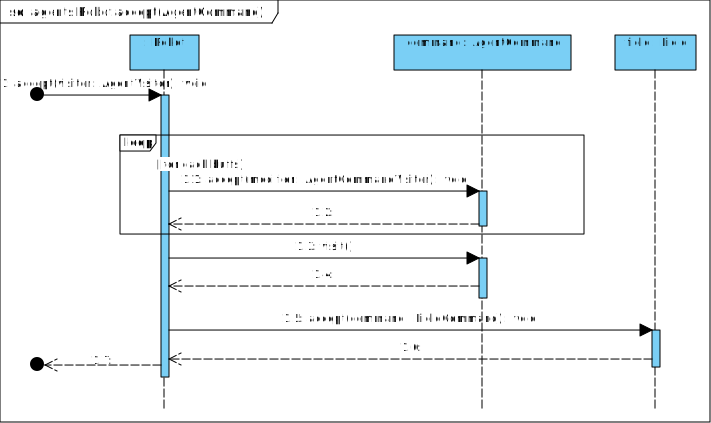
\includegraphics[width=\textwidth]{chapters/chapter03/agentsRobotacceptAgentCommand.pdf}
		\caption{Robot utasítást fogad}
		\label{fig:agents.Robot.accept}
	\end{center}
\end{figure}

\begin{figure}[h]
	\begin{center}
		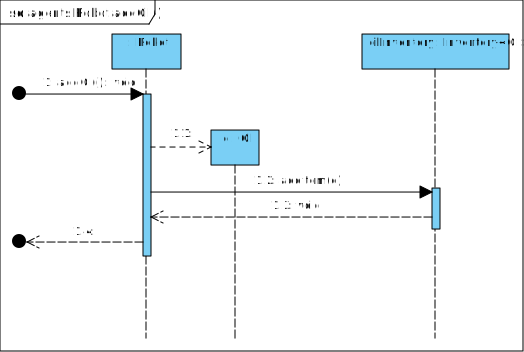
\includegraphics[width=\textwidth]{chapters/chapter03/agentsRobotaddOil.pdf}
		\caption{Robot felvesz a készletébe egy olajfoltot}
		\label{fig:agents.Robot.addOil}
	\end{center}
\end{figure}

\begin{figure}[h]
	\begin{center}
		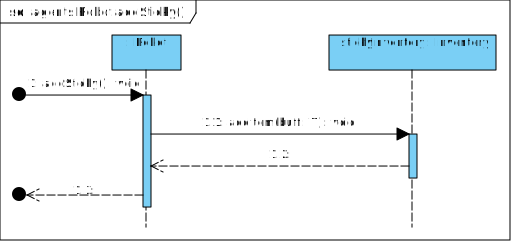
\includegraphics[width=\textwidth]{chapters/chapter03/agentsRobotaddSticky.pdf}
		\caption{Robot felvesz a készletébe egy ragacsfoltot}
		\label{fig:agents.Robot.addSticky}
	\end{center}
\end{figure}

\begin{figure}[h]
	\begin{center}
		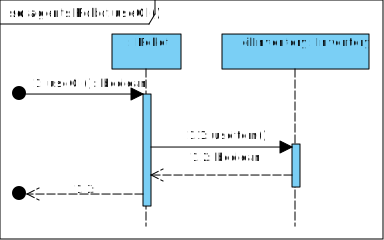
\includegraphics[width=\textwidth]{chapters/chapter03/agentsRobotuseOil.pdf}
		\caption{Robot felhasználja a készletében lévő olajfoltot ha van}
		\label{fig:agents.Robot.useOil}
	\end{center}
\end{figure}

\begin{figure}[h]
	\begin{center}
		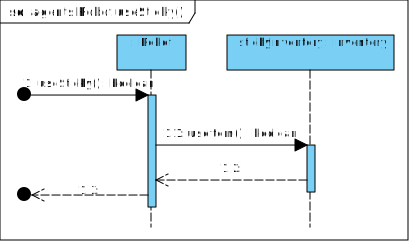
\includegraphics[width=\textwidth]{chapters/chapter03/agentsRobotuseSticky.pdf}
		\caption{Robot felhasználja a készletében lévő ragacsfoltot ha van}
		\label{fig:agents.Robot.useSticky}
	\end{center}
\end{figure}

\begin{figure}[h]
	\begin{center}
		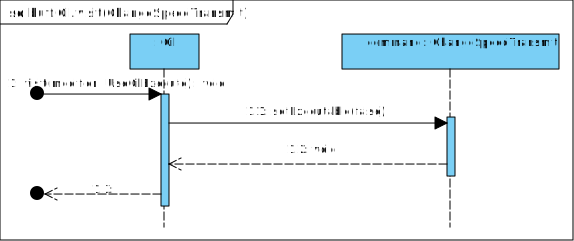
\includegraphics[width=\textwidth]{chapters/chapter03/buffOilvisitChangeSpeedTransmit.pdf}
		\caption{Olajfolt megakadályozza a sebesség nagyságának változtatását}
		\label{fig:buff.Oil.visit}
	\end{center}
\end{figure}

\begin{figure}[h]
	\begin{center}
		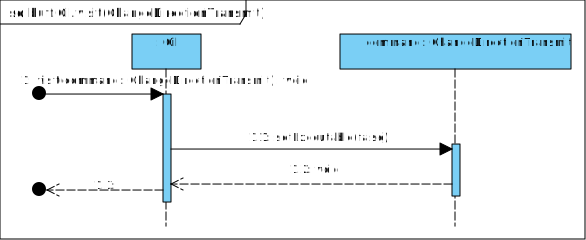
\includegraphics[width=\textwidth]{chapters/chapter03/buffOilvisitChangeDirectionTransmit.pdf}
		\caption{Olajfolt megakadályozza a sebesség irányának megváltoztatását}
		\label{fig:buff.Oil.visit2}
	\end{center}
\end{figure}

\begin{figure}[h]
	\begin{center}
		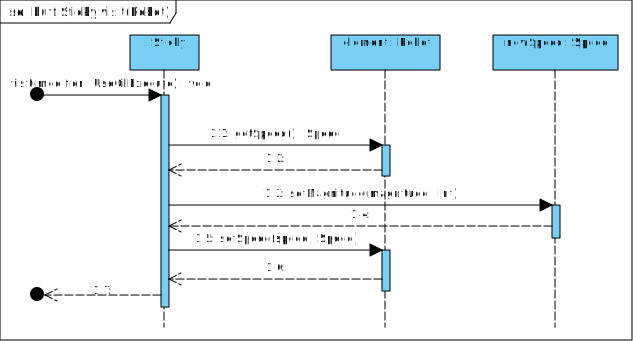
\includegraphics[width=\textwidth]{chapters/chapter03/buffStickyvisitRobot.pdf}
		\caption{Olajfolt megakadályozza a sebességváltoztatást}
		\label{fig:buff.Sticky.visit}
	\end{center}
\end{figure}

\begin{figure}[h]
	\begin{center}
		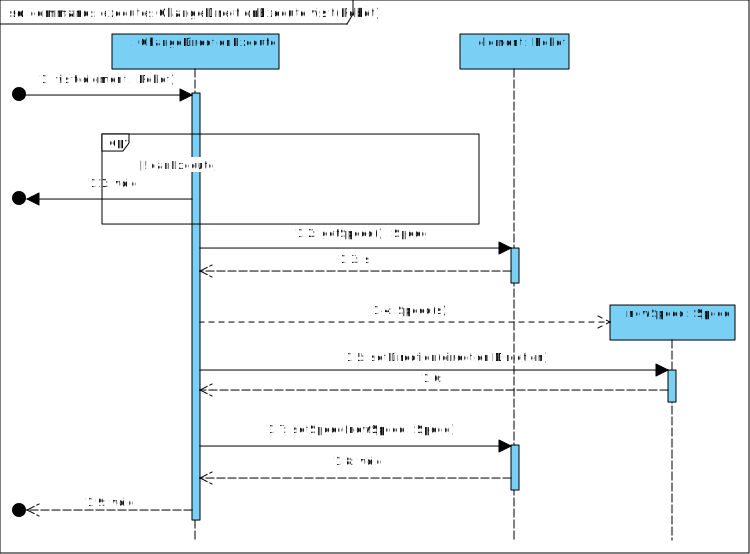
\includegraphics[width=\textwidth]{chapters/chapter03/commandsexecutesChangeDirectionExecutevisitRobot.pdf}
		\caption{Robot irányváltoztatásának végrehajtása}
		\label{fig:command.executes.ChangeDirectionExecute.visit}
	\end{center}
\end{figure}

\begin{figure}[h]
	\begin{center}
		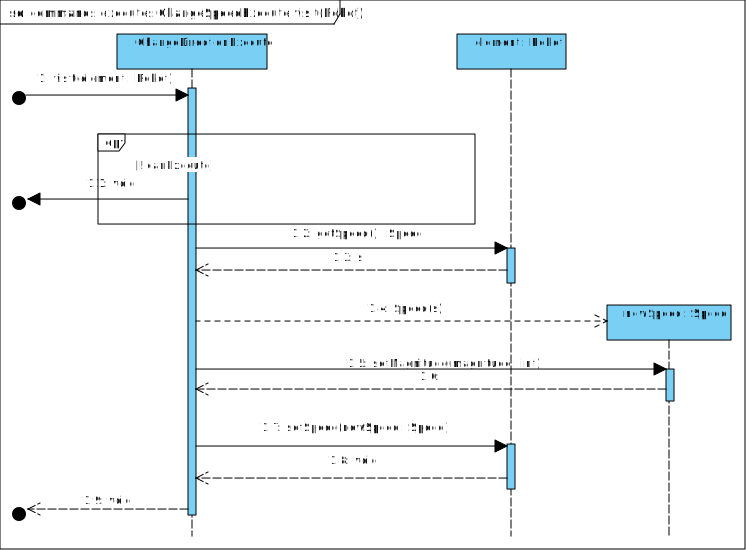
\includegraphics[width=\textwidth]{chapters/chapter03/commandsexecutesChangeSpeedExecutevisitRobot.pdf}
		\caption{Robot sebességnagyságának megváltoztatása}
		\label{fig:command.executes.ChangeSpeedExecute.visit}
	\end{center}
\end{figure}

\begin{figure}[h]
	\begin{center}
		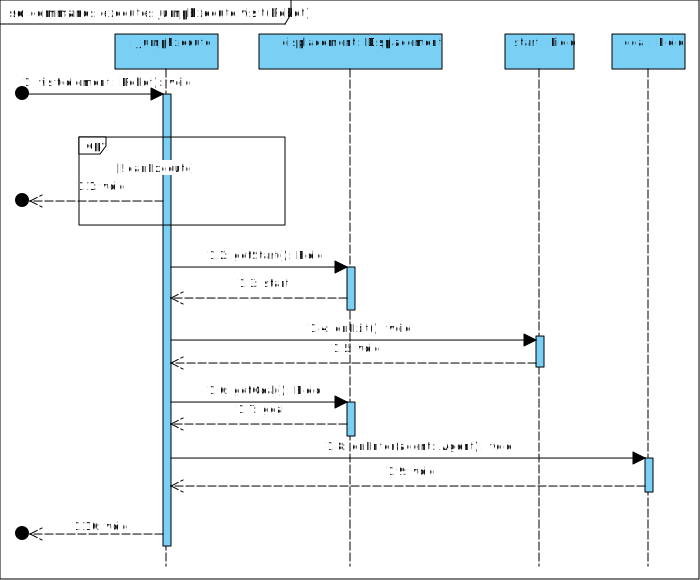
\includegraphics[width=\textwidth]{chapters/chapter03/commandsexecutesJumpExecutevisitRobot.pdf}
		\caption{Robot ugrásának végrehajtása}
		\label{fig:command.executes.JumpExecute.visit}
	\end{center}
\end{figure}

\begin{figure}[h]
	\begin{center}
		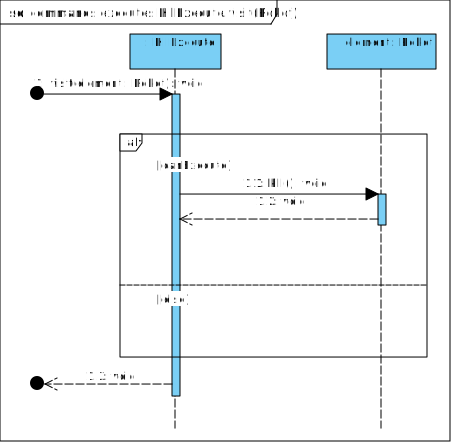
\includegraphics[width=\textwidth]{chapters/chapter03/commandsexecutesKillExecutevisitRobot.pdf}
		\caption{Robot megölésének végrehajtása}
		\label{fig:command.executes.KillExecute.visit}
	\end{center}
\end{figure}

\begin{figure}[h]
	\begin{center}
		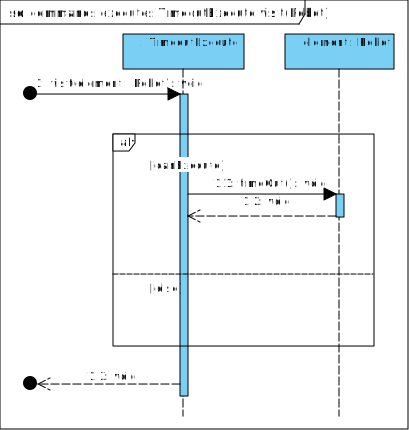
\includegraphics[width=\textwidth]{chapters/chapter03/commandsexecutesTimeoutExecutevisitRobot.pdf}
		\caption{Robot idő lejártának végrehajtása}
		\label{fig:command.executes.TimeoutExecute.visit}
	\end{center}
\end{figure}

\begin{figure}[h]
	\begin{center}
		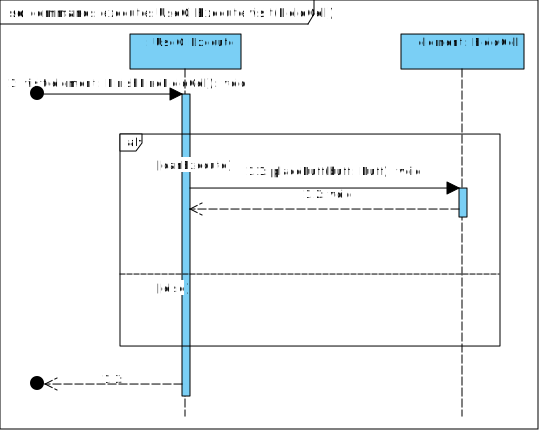
\includegraphics[width=\textwidth]{chapters/chapter03/commandsexecutesUseOilExecutevisitFieldCell.pdf}
		\caption{Robot lehelyezi az Olaj foltot a mezőre}
		\label{fig:command.executes.UseOilExecute.visit}
	\end{center}
\end{figure}

\begin{figure}[h]
	\begin{center}
		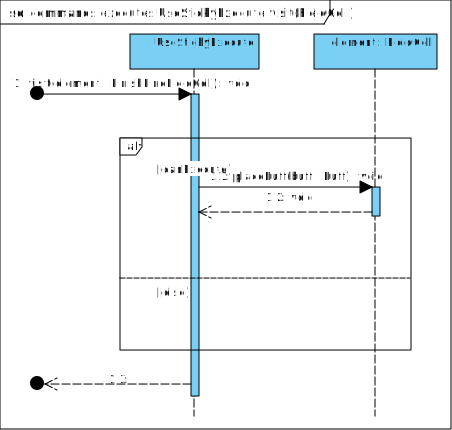
\includegraphics[width=\textwidth]{chapters/chapter03/commandsexecutesUseStickyExecutevisitFieldCell.pdf}
		\caption{Robot lehelyezi a Ragacs foltot a mezőre}
		\label{fig:command.executes.UseStickyExecute.visit}
	\end{center}
\end{figure}

\begin{figure}[h]
	\begin{center}
		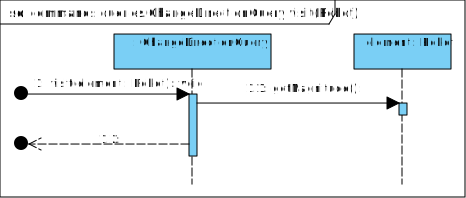
\includegraphics[width=\textwidth]{chapters/chapter03/commandsqueriesChangeDirectionQueryvisitRobot.pdf}
		\caption{Robot irányváltásra való felkérése}
		\label{fig:command.executes.ChangeDirectionQuery.visit}
	\end{center}
\end{figure}

\begin{figure}[h]
	\begin{center}
		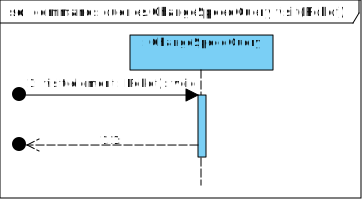
\includegraphics[width=\textwidth]{chapters/chapter03/commandsqueriesChangeSpeedQueryvisitRobot.pdf}
		\caption{Robot sebesség nagyságának megváltoztatására való felkérése}
		\label{fig:command.executes.ChangeSpeedQuery.visit}
	\end{center}
\end{figure}

\begin{figure}[h]
	\begin{center}
		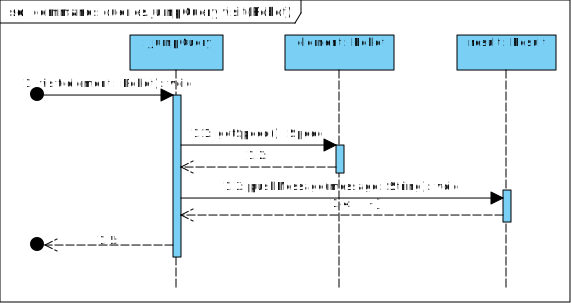
\includegraphics[width=\textwidth]{chapters/chapter03/commandsqueriesJumpQueryvisitRobot.pdf}
		\caption{Robot ugrásra azaz helyzetmódosításra való felkérése}
		\label{fig:command.executes.JumpQuery.visit}
	\end{center}
\end{figure}

\begin{figure}[h]
	\begin{center}
		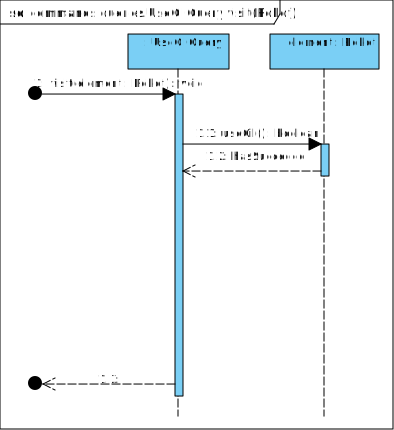
\includegraphics[width=\textwidth]{chapters/chapter03/commandsqueriesUseOilQueryvisitRobot.pdf}
		\caption{Robotot Olaj lehelyezésére való felkérése}
		\label{fig:command.executes.UseOilQuery.visit}
	\end{center}
\end{figure}

\begin{figure}[h]
	\begin{center}
		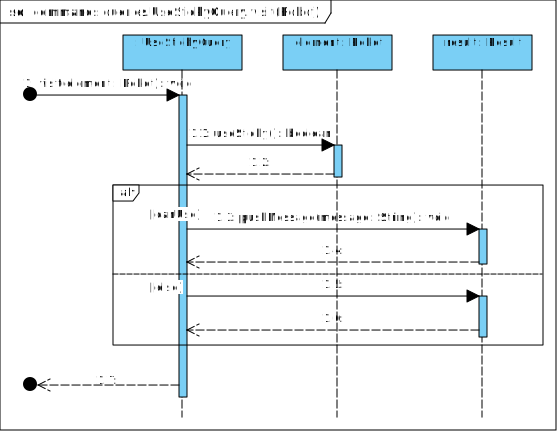
\includegraphics[width=\textwidth]{chapters/chapter03/commandsqueriesUseStickyQueryvisitRobot.pdf}
		\caption{Robotot Ragacs lehelyezésére való felkérése}
		\label{fig:command.executes.UseStickyQuery.visit}
	\end{center}
\end{figure}

\begin{figure}[h]
	\begin{center}
		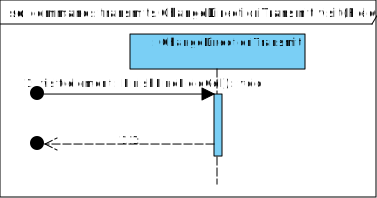
\includegraphics[width=\textwidth]{chapters/chapter03/commandstransmitsChangeDirectionTransmitvisitFieldCell.pdf}
		\caption{Irányváltásra vonatkozó kérés átvitele}
		\label{fig:command.executes.ChangeDirectionTransmit.visit}
	\end{center}
\end{figure}

\begin{figure}[h]
	\begin{center}
		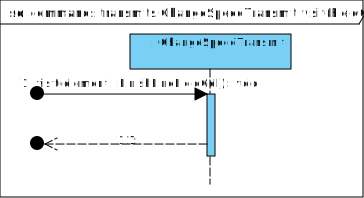
\includegraphics[width=\textwidth]{chapters/chapter03/commandstransmitsChangeSpeedTransmitvisitFieldCell.pdf}
		\caption{Szebességnagyság változtatásra vonatkozó kérés átvitele}
		\label{fig:command.executes.ChangeSpeedTransmit.visit}
	\end{center}
\end{figure}

\begin{figure}[h]
	\begin{center}
		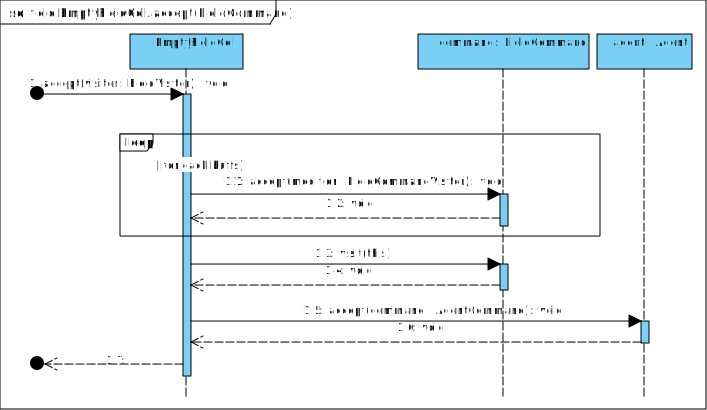
\includegraphics[width=\textwidth]{chapters/chapter03/fieldEmptyFieldCellacceptFieldCommand.pdf}
		\caption{Üres pályamező utasításfeldolgozása}
		\label{fig:field.EmptyFieldCell.accept}
	\end{center}
\end{figure}

\begin{figure}[h]
	\begin{center}
		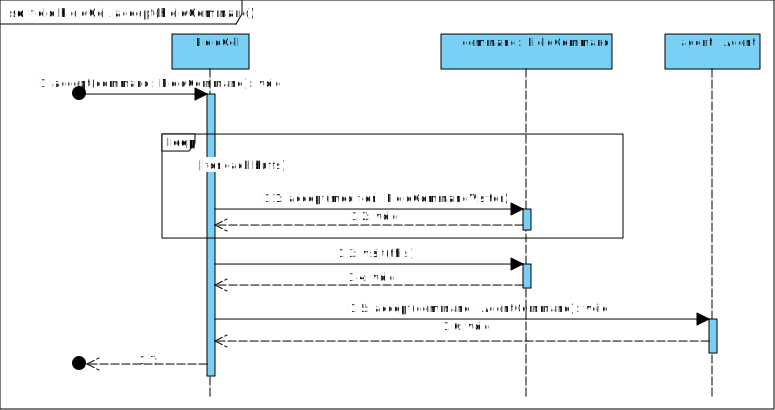
\includegraphics[width=\textwidth]{chapters/chapter03/fieldFieldCellacceptFieldCommand.pdf}
		\caption{Pályamező utasításfeldolgozása}
		\label{fig:field.FieldCell.accept}
	\end{center}
\end{figure}

\begin{figure}[h]
	\begin{center}
		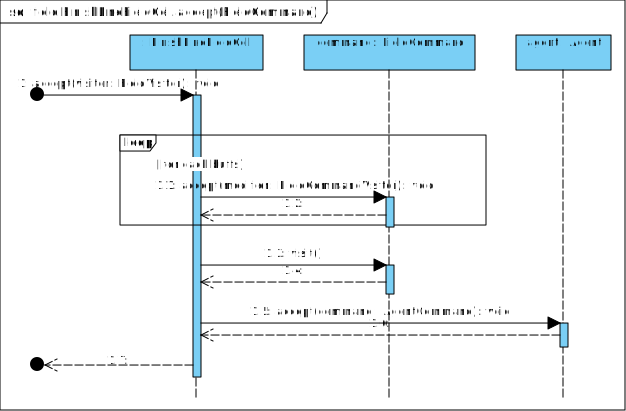
\includegraphics[width=\textwidth]{chapters/chapter03/fieldFinishLineFieldCellacceptFieldCommand.pdf}
		\caption{Start/célvonal pályamező utasításfeldolgozása}
		\label{fig:field.FinishLineFieldCell.accept}
	\end{center}
\end{figure}


\section{State-chartok}
\comment{Csak azokhoz az osztályokhoz, ahol van értelme. Egyetlen állapotból álló state-chartok ne szerepeljenek. A játék működését bemutató state-chart-ot készíteni tilos.}

\begin{figure}[h]
\begin{center}
%\includegraphics[width=17cm]{chapters/chapter03/example.pdf}
\caption{x}
\label{fig:example3}
\end{center}
\end{figure}

